\documentclass[a4paper,11pt,UTF8]{article}
\usepackage{ctex}
\usepackage{amsmath,amsthm,amssymb,amsfonts}
\usepackage{amsmath}
\usepackage[a4paper]{geometry}
\usepackage{graphicx}
\usepackage{microtype}
\usepackage{siunitx}
\usepackage{booktabs}
\usepackage[colorlinks=false, pdfborder={0 0 0}]{hyperref}
\usepackage{cleveref}
\usepackage{esint} 
\usepackage{graphicx}
\usepackage{ragged2e}
\usepackage{pifont}
\usepackage{extarrows}
\usepackage{mathptmx}
\usepackage{float}
\usepackage{caption}
\usepackage{multirow}
\usepackage{subfigure}
\usepackage{titlesec}
\titleformat{\section}{\Large\bfseries}{\chinese{section}、}{0em}{}
\titleformat{\subsection}{\large\bfseries}{\thesubsection}{0em}{}
\titleformat{\subsubsection}{\normalsize\bfseries}{\thesubsubsection}{1em}{}

\begin{document}
	
\title{\huge 实验报告 \\ 集成运算放大器在信号运算方面的应用}
\author{电子信息与通信学院 \\ 提高2301班 \\ 张禹阳 \ U202314270}

\maketitle

\begin{figure}[H]
	\centering
	\subfigure{
		
\includegraphics[scale=1]{hust.png}
	}
	\subfigure{
		
\includegraphics[scale=1]{eic.png}
	}
\end{figure}

\tableofcontents

\section{实验目的}
熟练安装、调试本节介绍的由运放构成的基本运算电路,熟练掌握它们的工作原理,掌握运放电路的基本分析

\section{实验元器件}
运算放大器NE5532,
100$\mathrm{\Omega}$电阻,
500$\mathrm{\Omega}$电阻,
1$\mathrm{k\Omega}$电阻,
5.1$\mathrm{k\Omega}$电阻,
10$\mathrm{k\Omega}$电阻,
100$\mathrm{k\Omega}$电阻

\section{实验任务}

\subsection{ \ 任务1: 研究电压跟随器的作用}
测试下图所示两种电路各电压幅值,观察有、无电压跟随器的差别

\subsubsection{实验原理及电路}

\begin{figure}[H]
	\centering
	\setcounter{subfigure}{0}
	\subfigure[直接连接]{
		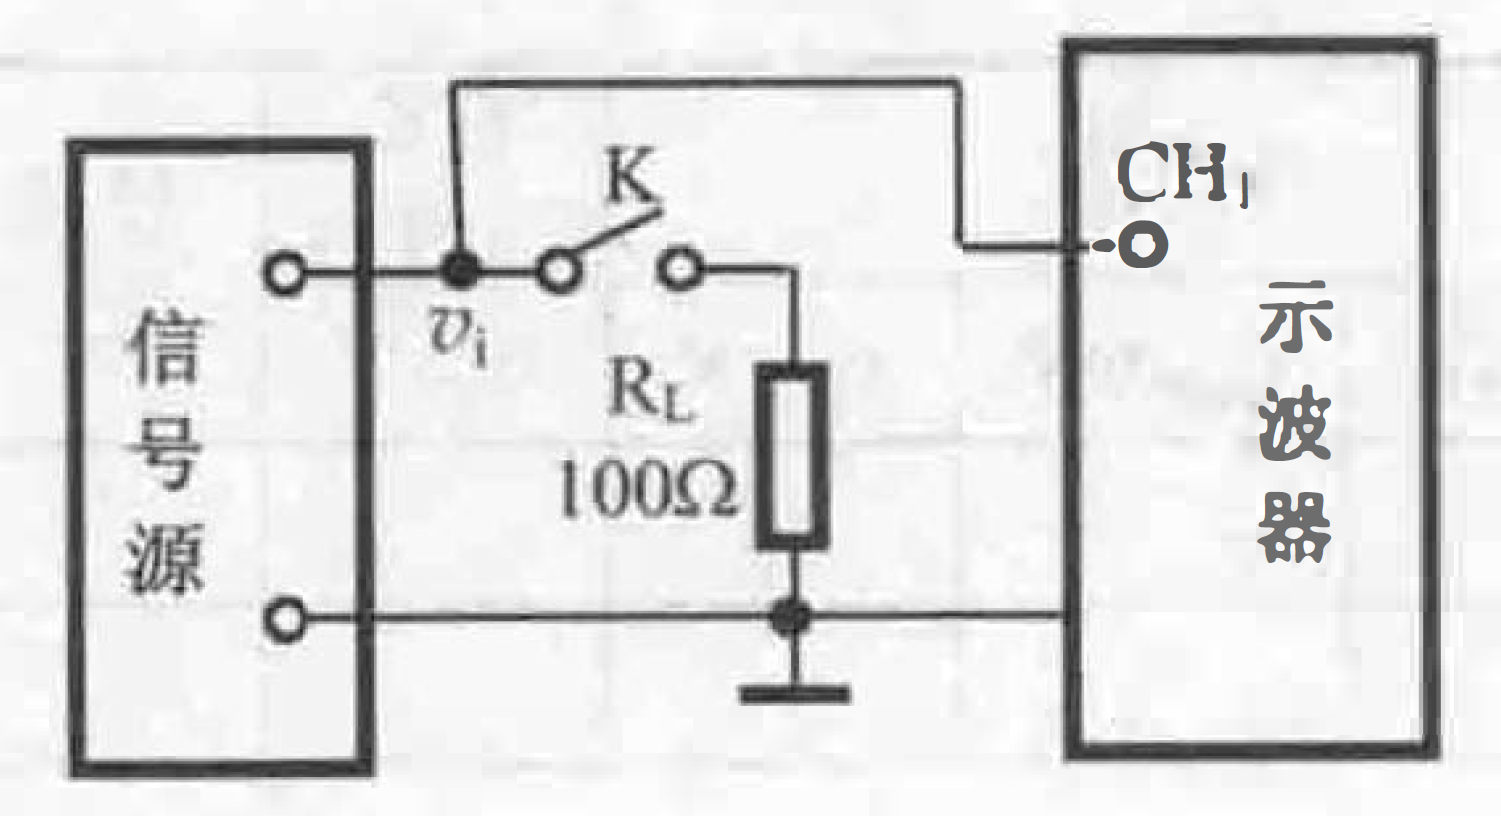
\includegraphics[scale=0.1]{1.1.png}
		\label{fig:subfig1}		
	}
	\subfigure[通过电压跟随器连接]{
		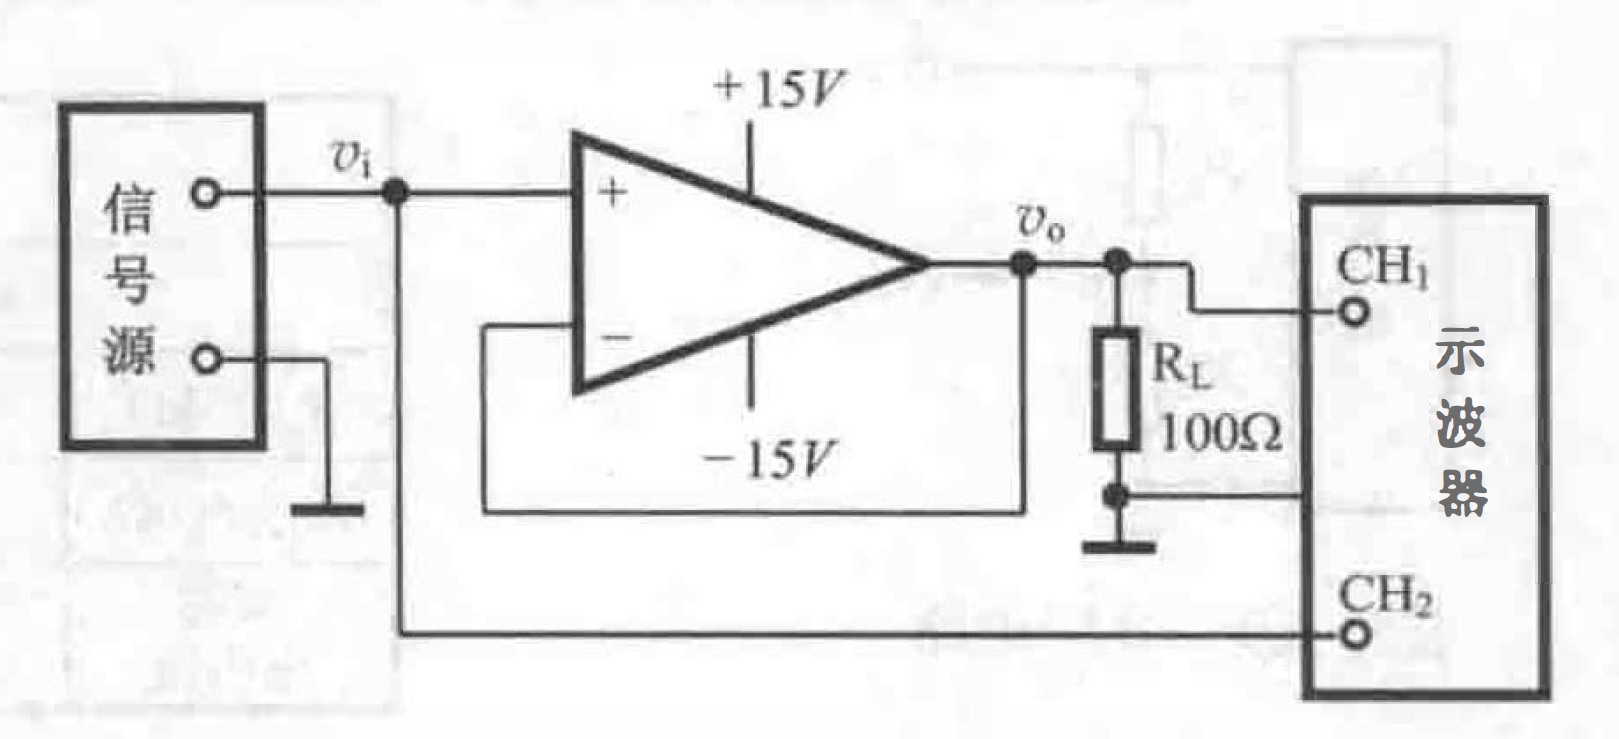
\includegraphics[scale=0.12]{1.2.png}
	}
	\caption{信号源与负载连接}
\end{figure}

\subsubsection{实验过程}

(1) 按照图 (a) 在面包板上组装电路

(2) 从信号源送出频率为1kHz、峰-峰值为1V的正弦信号。不接负载 $R_L$(K断开)时,用示波器观测 $v_i$ 
波形并填入下表中;接入负载 $R_L$(K闭合)时,用示波器观测 $v_i$ 波形并填入下表中

(3) 按照图(b)连接电路,仍从信号源送出频率为1kHz、峰-峰值为1V的正弦信号,用示波器两个通道同时观察
输入、输出波形,分别测量未接 $R_L$ 和接入 $R_L$ 两种情况下 $v_i$ 和 $v_io$ 的大小并填入下表中

(4) 计算信号源的内阻 $R_S$,说明100 $\Omega$ 负载电阻连接到信号源上产生的负载效应,并解释观察到
的实验现象

\begin{table}[h]
	\centering
	\caption{电压跟随器的作用数据记录表格}
	\label{table1}
	\begin{tabular}{|c|c|c|c|c|c|}
		\hline
		\multirow{2}{*}{}   & \multicolumn{2}{c|}{不接$R_L$} & \multicolumn{2}{c|}{接入$R_L$} &
		\multirow{2}{*}{计算$R_s/\Omega$}\\
		\cline{2-5}
		\multirow{2}{*}{} & $v_{ipp}/$V & $v_{opp}/$V & $v_{ipp}/$V & $v_{opp}/$V & \multirow{2}{*}{}\\
		\hline
		无电压跟随器 &  & - &  & - &  \\
		\hline
		有电压跟随器 &  &  &  &  & - \\
		\hline
	\end{tabular}
\end{table}

信号源的内阻计算可以按照分压公式计算:
$$
	R_s=\frac{V_s-v_{ipp(R_L)}}{v_{ipp(R_L)}}R_L
$$

\subsection{ \ 任务2: 反相比例加法运算电路测试}
测试下图所示反相比例加法器的输入输出电压,验证它们的运算关系

\subsubsection{实验原理及电路}
根据运放的虚短和虚断特性,可求得其输出电压为:
$$
	V_0=-\left(\frac{R_{\mathrm{F}}}{R_1}V_1+\frac{R_{\mathrm{F}}}{R_2}V_2\right)
$$

\begin{figure}[H]
	\centering
	\subfigure[分压电路]{
		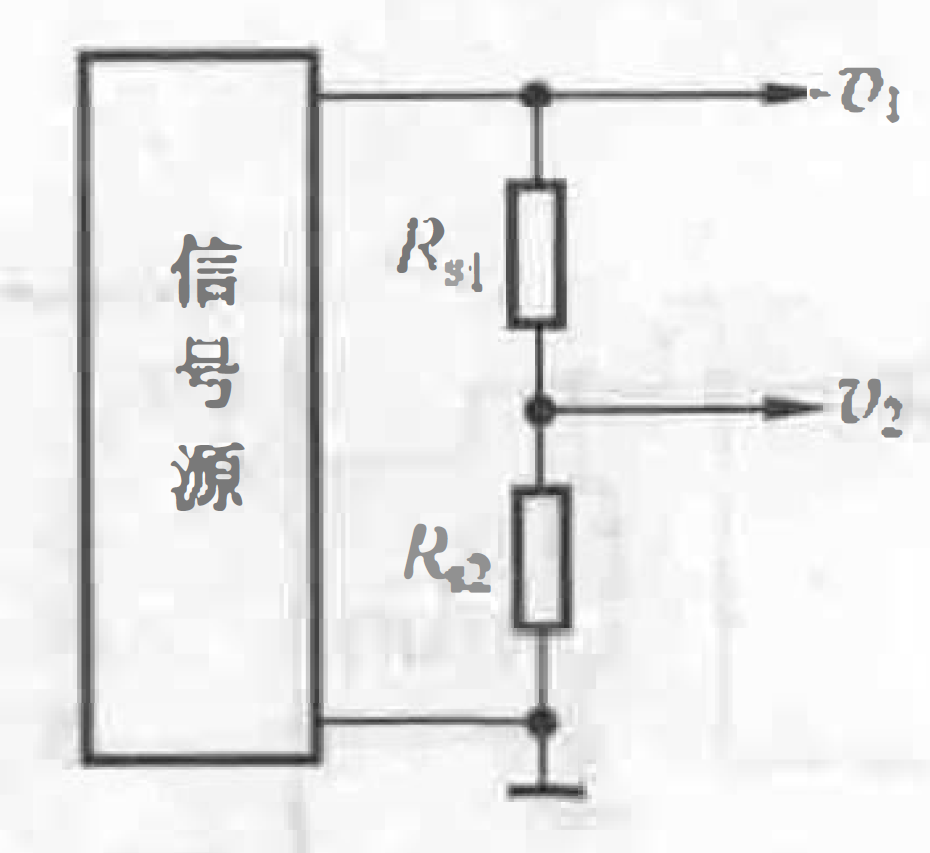
\includegraphics[width=0.45\textwidth]{1.3.2.png}
	}
	\subfigure[实验电路图]{
		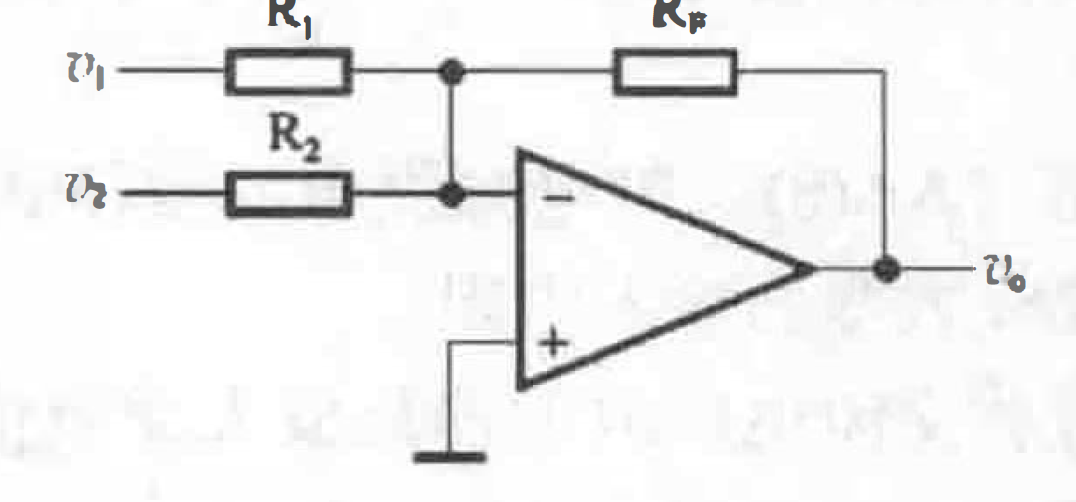
\includegraphics[width=0.45\textwidth]{1.3.1.png}
	}
	\caption{反向比例加法器}
\end{figure}

\subsubsection{实验过程}

(1) 按照上图在面包板上组装电路。电阻值取 $R_F = 100k\Omega$,$R_1 = 10k\Omega$,
$R_2 = 5.1k\Omega$,安装电阻前先用万用表测试电阻值填入表中

(2)按照上图连接分压电路和实验电路,其中 $R_{s1} = R_{s2} = 1k\Omega$。从信号源送出频率为
1kHz、峰-峰值为300mV的正弦信号。用示波器测得 $v_1,v_2$ 和 $v_o$。填入下表中,并记录它们的波形

(3)关闭电源,将 $Rs2$ 改为500 $\Omega$,检查无误后接通电源,再次用示波器测得 $v_1,v_2$ 
和 $v_o$。填入下表中

\begin{table}[h]
	\centering
	\caption{加法器实验数据表格}
	\label{table2}
	\begin{tabular}{|c|c|c|c|c|c|c|}
		\hline
		\multirow{2}{*}{}   & \multicolumn{3}{c|}{实测值} & 理论值 &
		\multirow{2}{*}{相对误差} & 
		\multirow{2}{*}{绝对误差}\\
		\cline{2-5}
		\multirow{2}{*}{} & $v_{1pp}$/mV & $v_{2pp}/$/mV & $v_{opp}$/V & $v_{opp}$/V & 
		\multirow{2}{*}{} &
		\multirow{2}{*}{}\\
		\hline
		$R_{s2}=1\mathrm{k\Omega}$ &  &  &  &  &  &  \\
		\hline
		$R_{s2}=500\mathrm{\Omega}$ &  &  &  &  &  &  \\
		\hline
		实测电阻值 & \multicolumn{6}{c|}{$R_1= \ \ \ ,R_2= \ \ \ , R_F=$}\\
		\hline
	\end{tabular}
\end{table}

\subsection{ \ 任务3: 比例积分电路测试}
测试下图所示比例积分器的输入、输出波形

\subsubsection{实验原理及电路}
当$R_F\gg R_1$时,电路的输出电压可近似为:
$$
	v_{\mathrm{o}}(t)=-\frac{1}{R_{1}C}\int_{0}^{t}v_{\mathrm{i}}(t)\mathrm{d}t+v_{\mathrm{o}}(0)
$$

\begin{figure}[H]
	\centering
	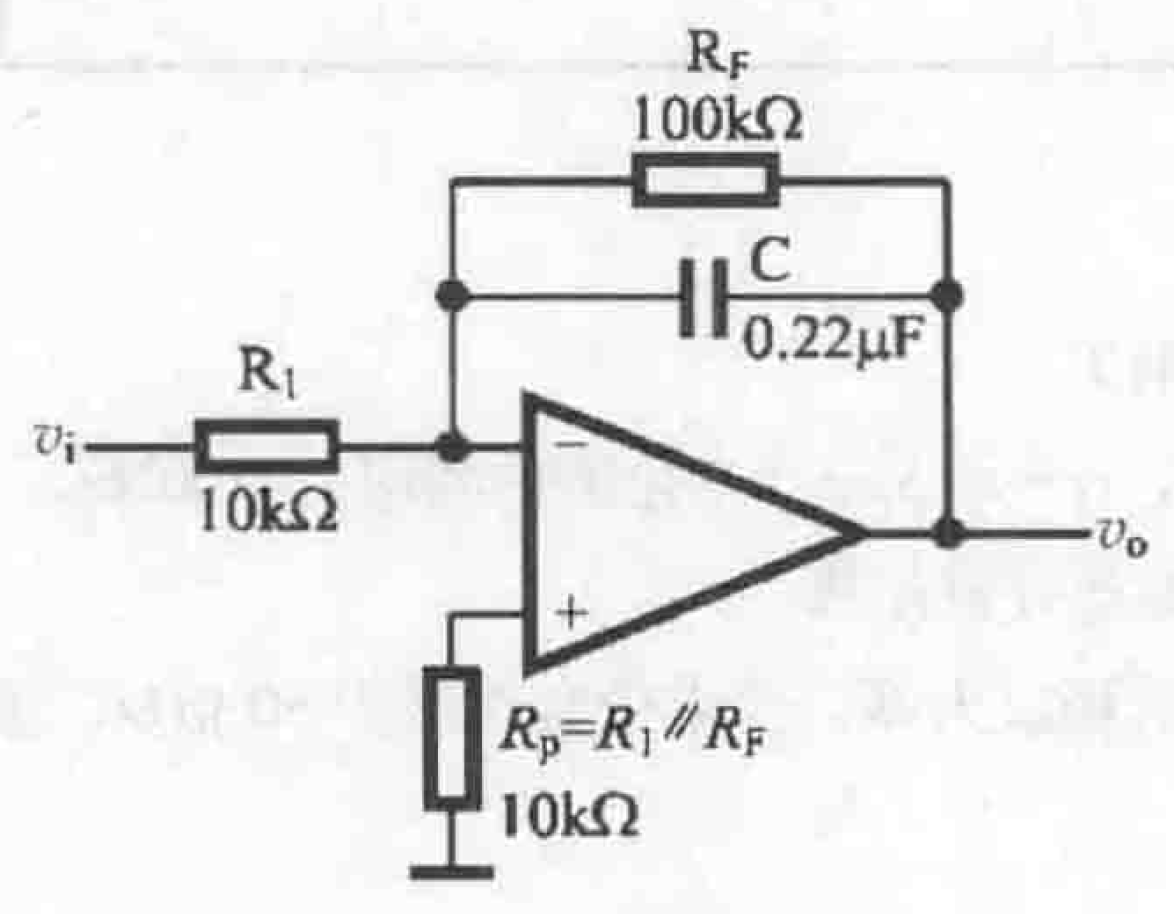
\includegraphics[scale=0.18]{1.4.png}
	\caption{比例积分电路}
\end{figure}

\subsubsection{实验过程}
从信号源送出 200Hz、1V 的正方波作为 $v_\mathrm{i}$,用示波器两个通道同时
观测$v_\mathrm{i}$和$v_\mathrm{o}$,并定量画出它们的波形(需含有坐标轴,波形上下对齐)

\subsection{ \ 任务4: 研究交流仪表放大器的性能}
选取电路参数,设计一个电压增益大于500倍的交流仪表放大器,测量电路的差模电压增益、共模抑制比和
差模电压增益的幅频响应

\subsubsection{实验原理及电路}
当选择 $R_1 = R_2, R_3 = R_4, R_5 = R_6, R_F = R_7$ 时,电压增益为:
$$
A_{VD} = \frac{V_o}{V_2 - V_1} = (1+\frac{R_3 + R_4}{R})\frac{R_F}{R_5}
$$
当测量差模电压增益时,由于同时有共模信号输入,计算根据:
$$
A_{VD} = |\frac{v_{opp}}{v_{2pp}-v_{1pp}}|-\frac{v_{2pp}+v_{1pp}}{2(v_{2pp} - v_{1pp})} \cdot A_{VC}
$$

\begin{figure}[H]
	\centering
	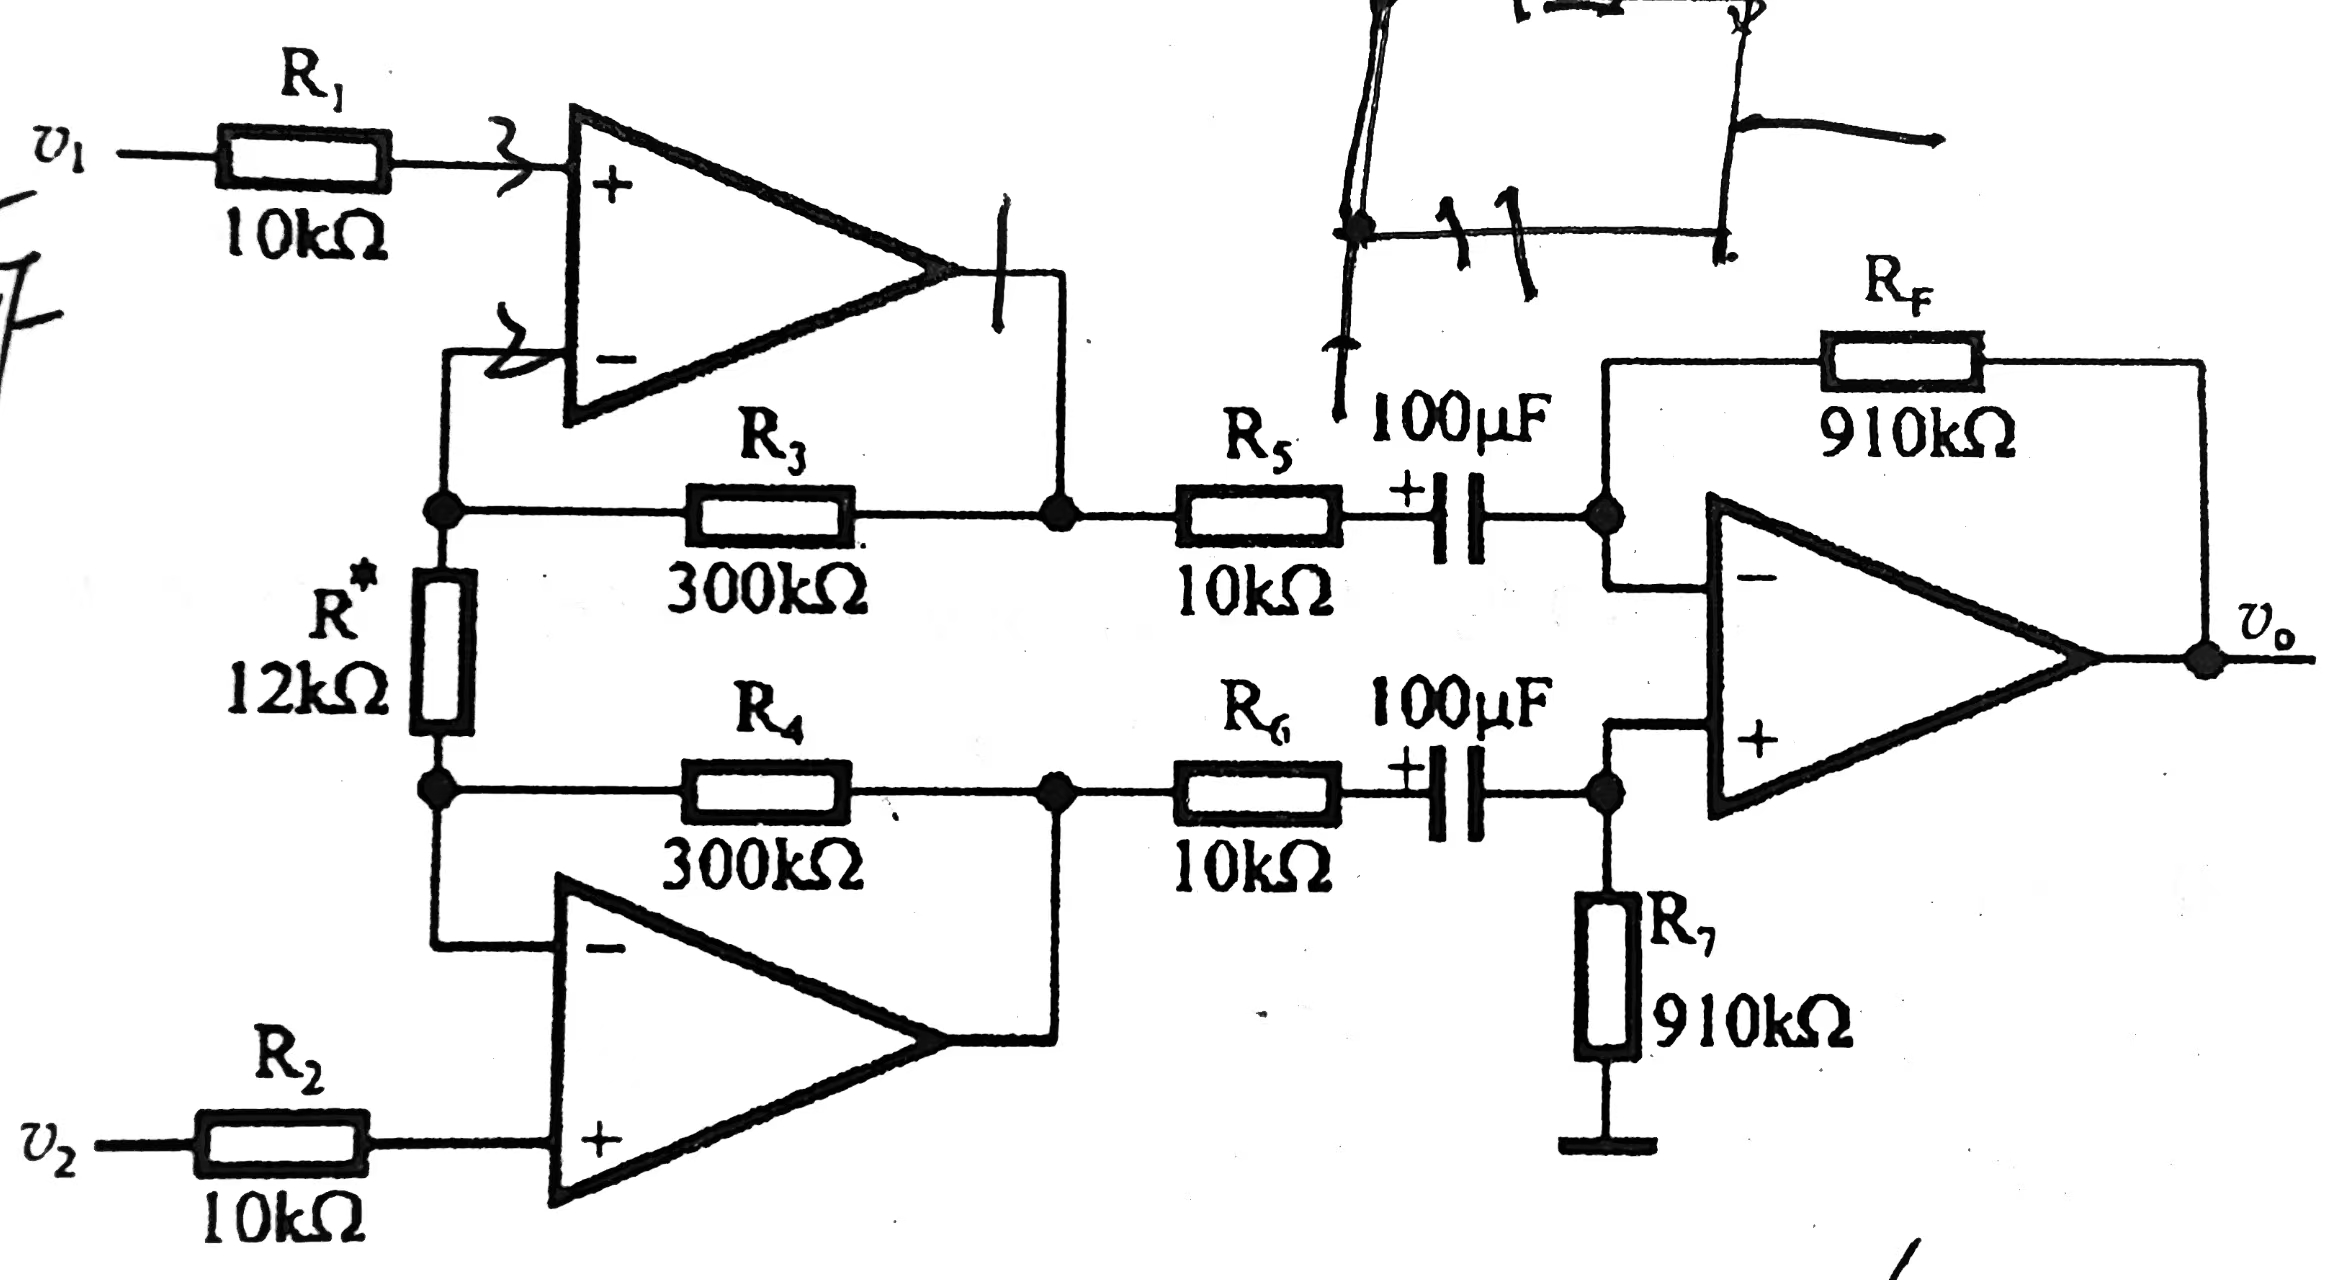
\includegraphics[scale=0.18]{1.11.jpg}
	\caption{交流仪表放大器}
\end{figure}

\subsubsection{实验过程}

(1) 将电路组装在面包板上
(2) 测量共模电压增益 $A_{VC}$。将 $v_1$ 和 $v_2$ 并联,作为共模电压 $v_{ic}$ 的输入端。
$v_{ic}$ 输入频率为 500Hz、峰-峰值为 10V 的正弦波,用示波器两个通道同时观察 $v_{ic}$ 和
$v_{oc}$,并计算带相位关系的共模电压增益
(3) 测量差模电压增益 $A_{VD}$ 并计算共模抑制比。按任务二中分压电路接法连接,其中 
$R_{s1} = R_{s2} = 1k\Omega$。从信号源送出频率为 500Hz、峰-峰值为 100mV 的正弦波
(4) 测量 $A_{VD}$ 的幅频响应。保持输入信号电压不变,调节信号源频率,不断升高信号频率,观察
输出波形的幅值变化,测出其上限频率

\section{实验分析}

\subsection{任务1: 研究电压跟随器的作用}
观察到的波形如下:

\begin{figure}[H]
	\centering
	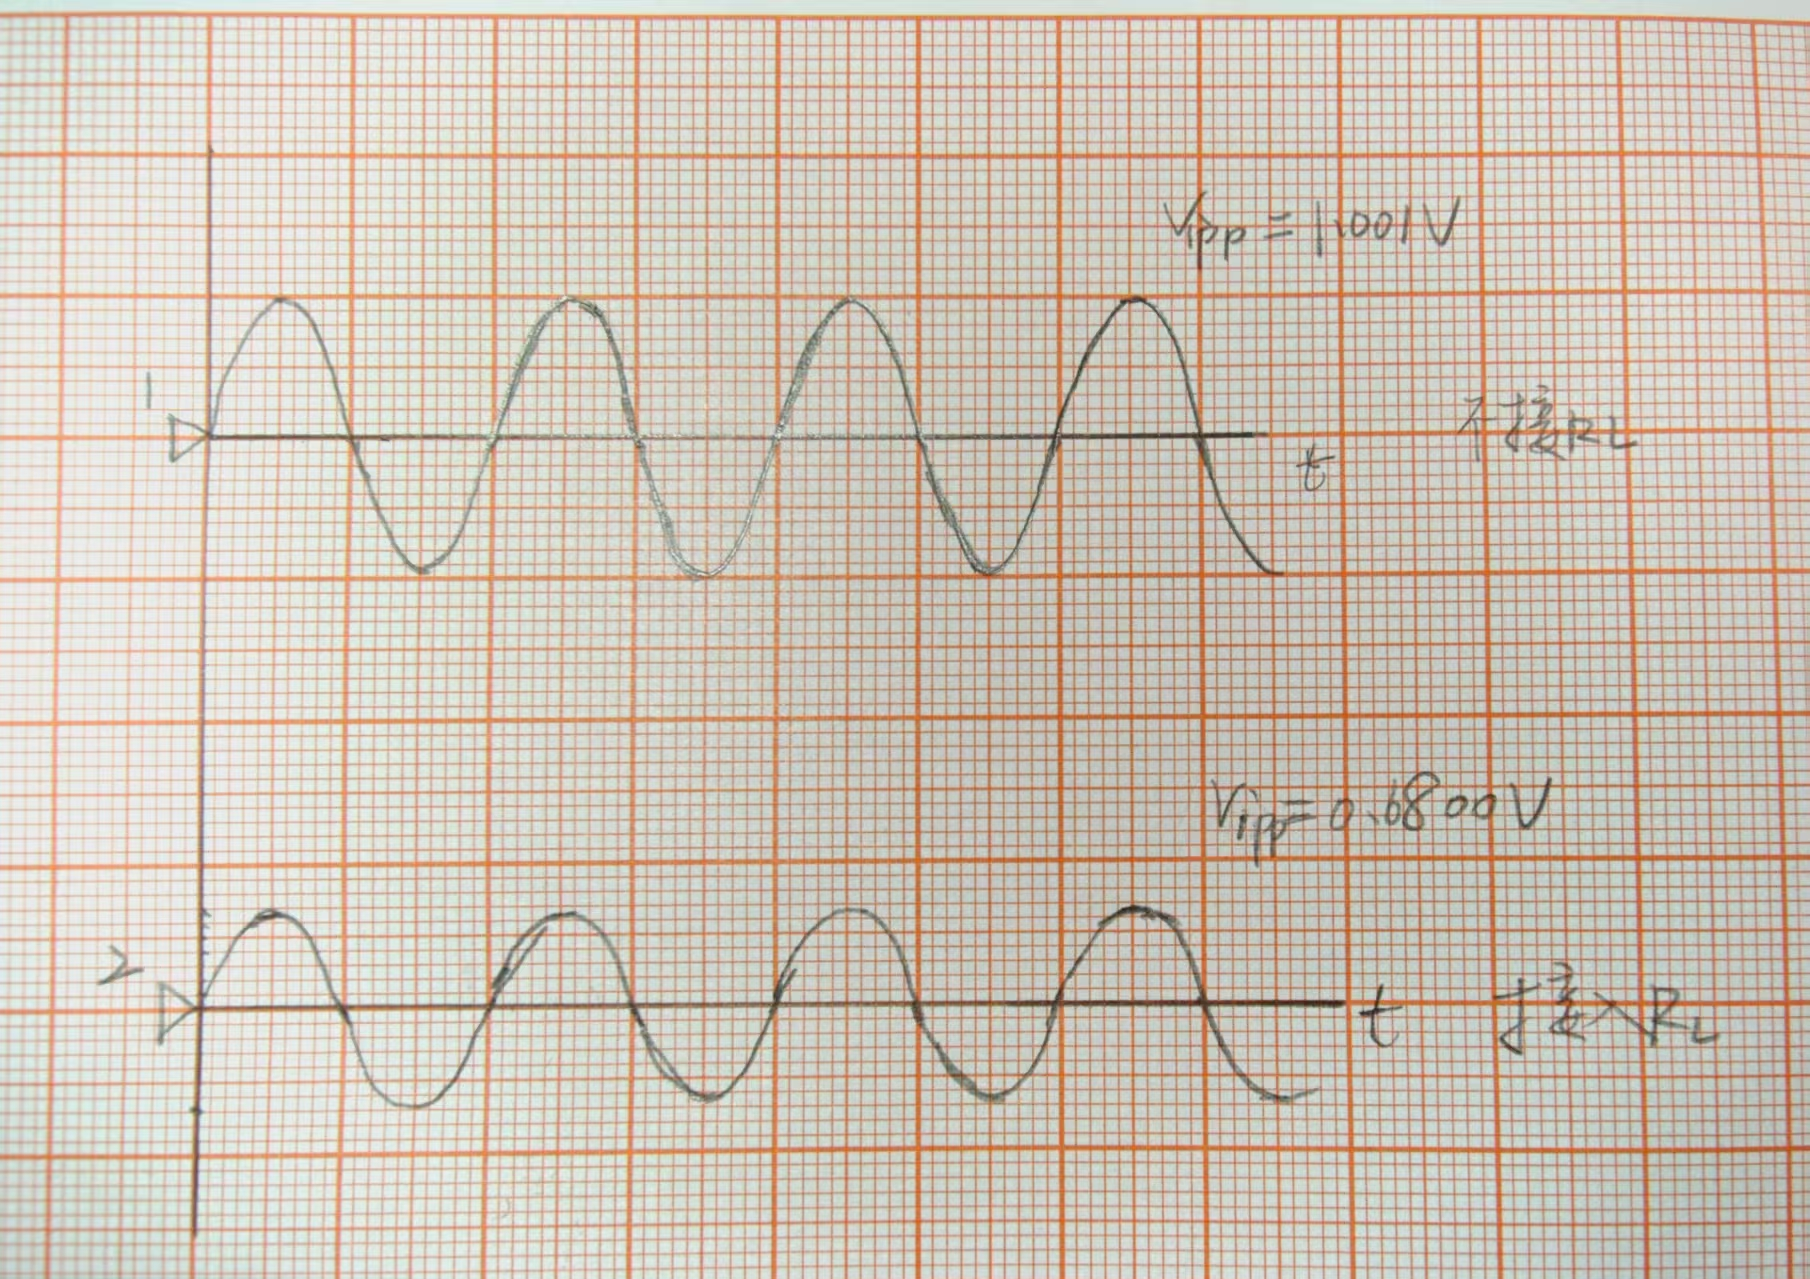
\includegraphics[width = 0.8\textwidth]{1.5.jpg}
	\caption{无电压跟随器}
\end{figure}

\begin{figure}[H]
	\centering
	\setcounter{subfigure}{0}
	\subfigure[不接 $R_L$]{
		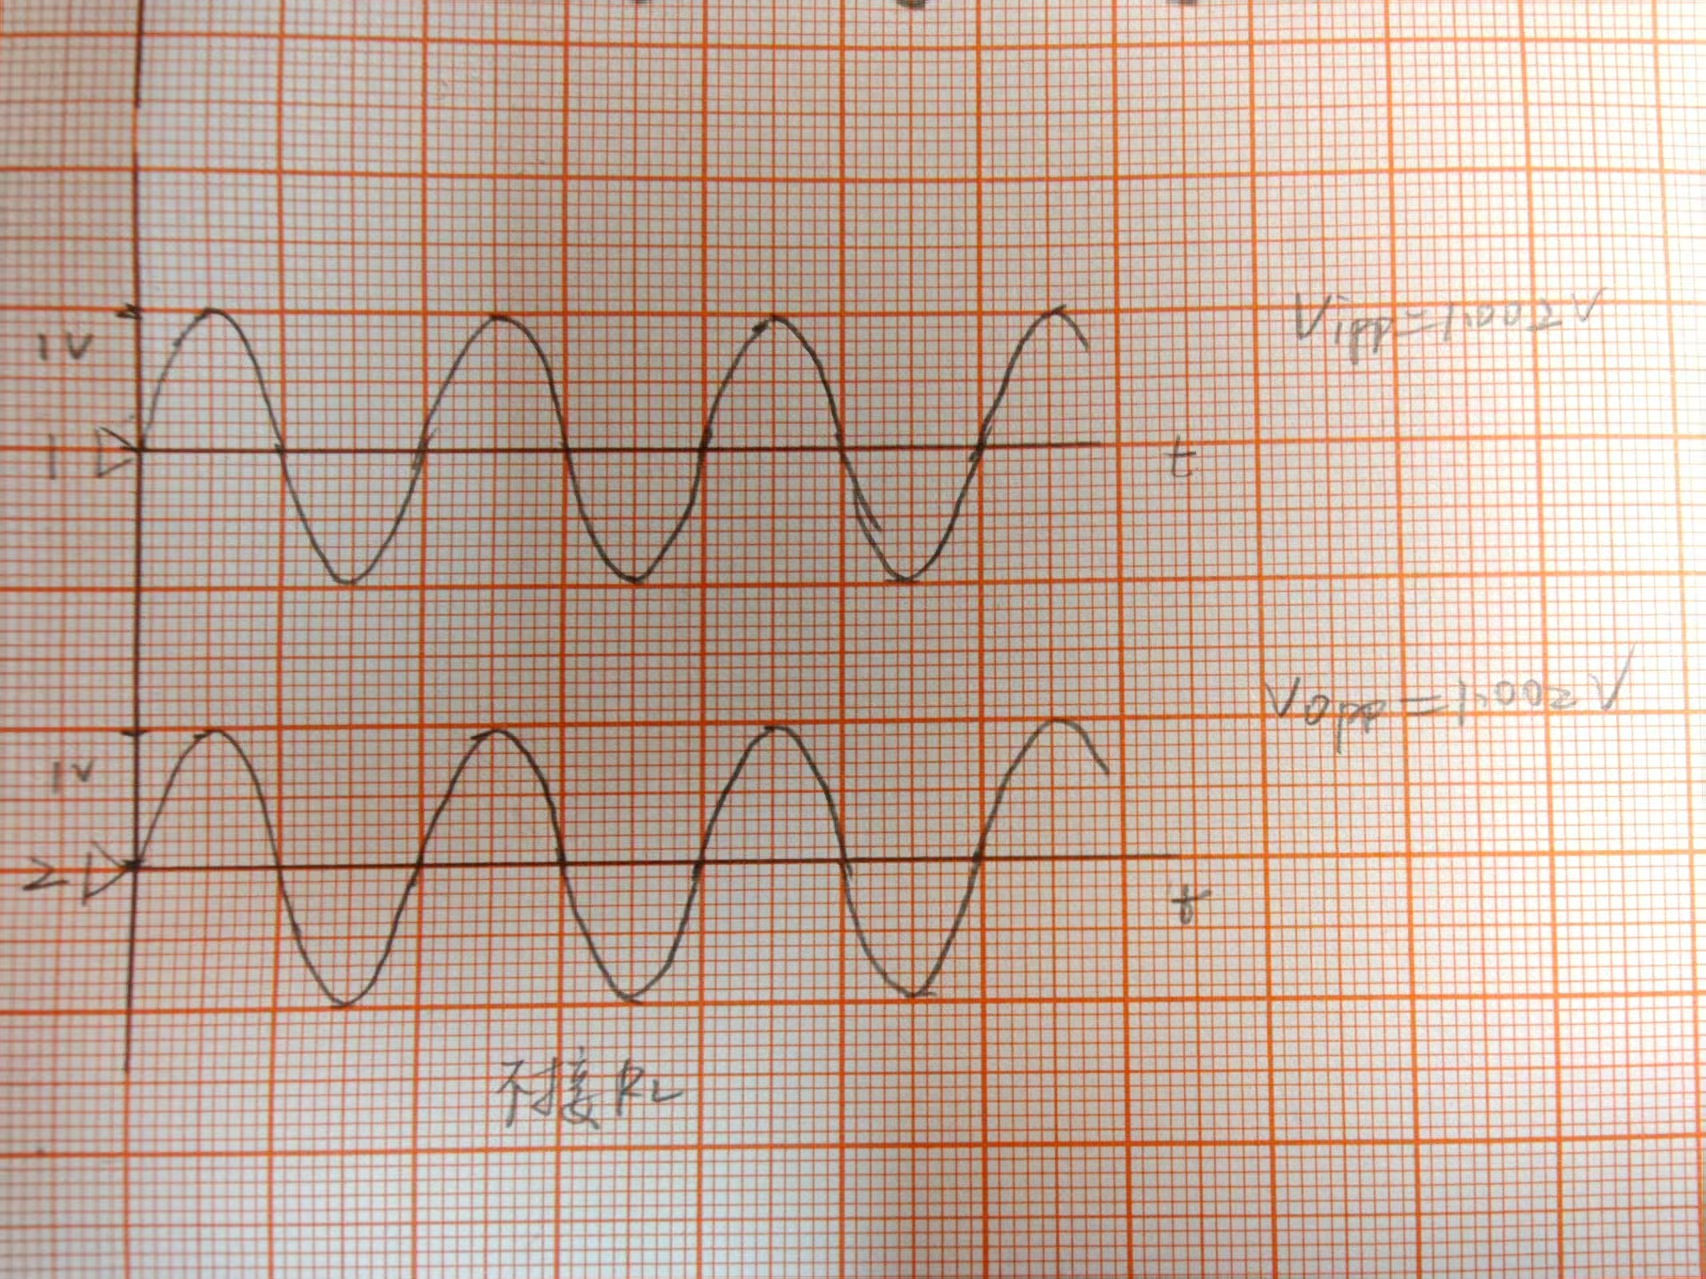
\includegraphics[width = 0.45\textwidth]{1.6.jpg}
	}
	\subfigure[接入 $R_L$]{
		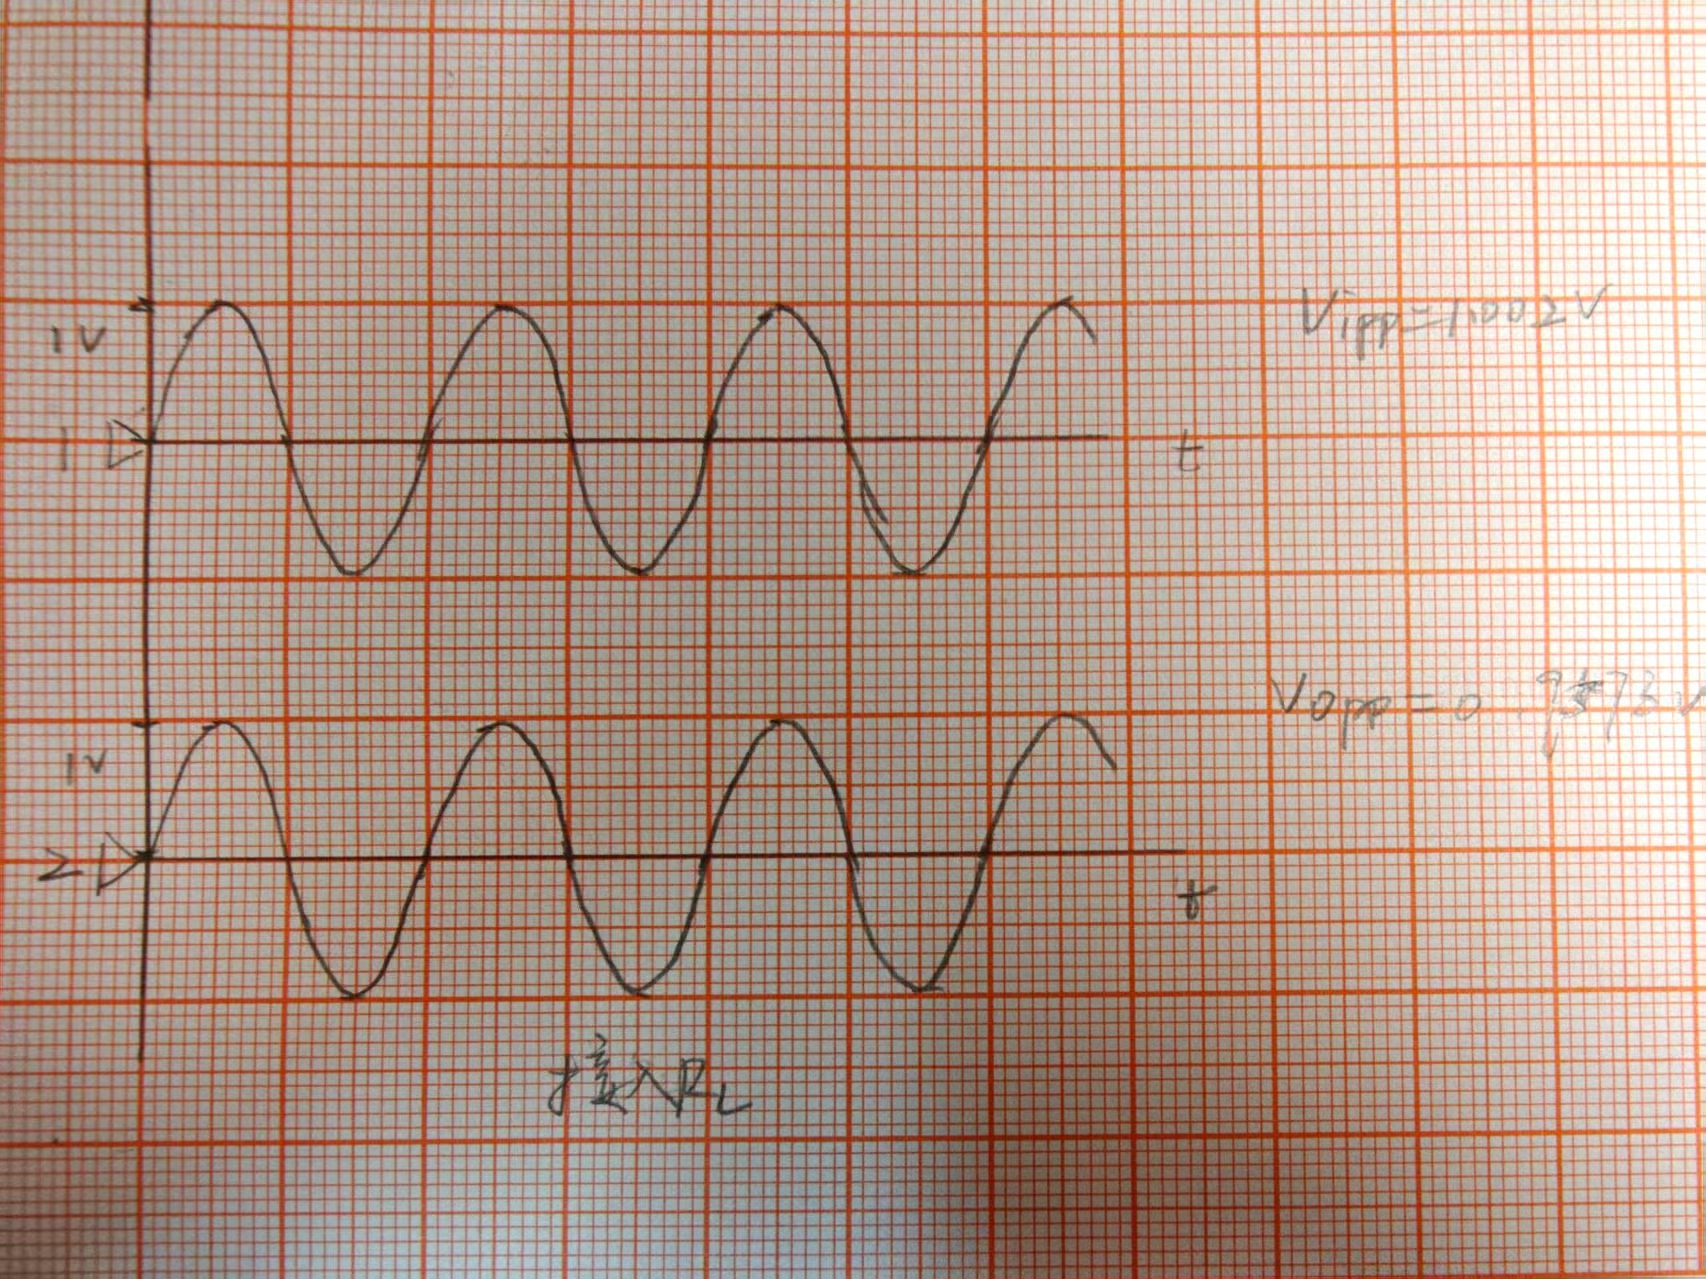
\includegraphics[width = 0.45\textwidth]{1.7.jpg}
	}
	\caption{有电压跟随器}
\end{figure}

可以看到在缺少电压跟随器时,接入$R_L$后电压下降明显,并根据分压公式计算出了信号源内阻。
负载效应是指由于负载电阻的存在,导致信号源输出电压产生电压降。由于负载电阻的存在,
信号源的输出电压会在连接负载时产生降低。根据欧姆定律,当电流经过电阻时,会产生电压降。
因此,连接100Ω负载电阻后,信号源输出电压会相应降低。

数据记录表格如下:

\begin{table}[h]
	\centering
	\caption{电压跟随器数据记录表格}
	\label{label3}
	\begin{tabular}{|c|c|c|c|c|c|}
		\hline
		\multirow{2}{*}{}   & \multicolumn{2}{c|}{不接$R_L$} & \multicolumn{2}{c|}{接入$R_L$} &
		\multirow{2}{*}{计算$R_s/\Omega$}\\
		\cline{2-5}
		\multirow{2}{*}{} & $v_{ipp}/$V & $v_{opp}/$V & $v_{ipp}/$V & $v_{opp}/$V & \multirow{2}{*}{}\\
		\hline
		无电压跟随器 & 1.001 & - & 0.6800 & - & 47.06\\
		\hline
		有电压跟随器 & 1.002 & 1.002 & 1.003 & 0.9573 & - \\
		\hline
	\end{tabular}
\end{table} 

\subsection{任务2: 反相比例加法运算电路测试}
实验数据如下,误差在5\%~6\%左右,属于比较合理的实验误差:

\begin{table}[htbp]
	\centering
	\caption{加法器实验数据表格}
	\label{label4}
	\begin{tabular}{|c|c|c|c|c|c|c|}
		\hline
		\multirow{2}{*}{}   & \multicolumn{3}{c|}{实测值} & 理论值 &
		\multirow{2}{*}{相对误差} &
		\multirow{2}{*}{绝对误差}\\
		\cline{2-5}
		\multirow{2}{*}{} & $v_{1pp}$/mV & $v_{2pp}/$/mV & $v_{opp}$/V & $v_{opp}$/V & 
		\multirow{2}{*}{} & 
		\multirow{2}{*}{} \\
		\hline
		$R_{s2}=1\mathrm{k\Omega}$ & 294.0 & 136.3 & 5.486 & 5.942 & 7.7\% & 0.456 \\
		\hline
		$R_{s2}=500\mathrm{\Omega}$ & 292.0 & 93.60 & 4.630 & 4.961 & 6.7\% & 0.331 \\
		\hline
		实测电阻值 & \multicolumn{6}{c|}{$R_1=9.8213\mathrm{k\Omega},R_2=5.0148\mathrm{k\Omega}, R_F=99.087\mathrm{k\Omega}$}\\
		\hline
	\end{tabular}
\end{table}

观察到的波形如下:

\begin{figure}[H]
	\centering
	\setcounter{subfigure}{0}
	\subfigure[$v_{1pp}$,$v_{2pp}$ 和 $v_{opp}$ ($R_{s2}= 1k\Omega$)]{
		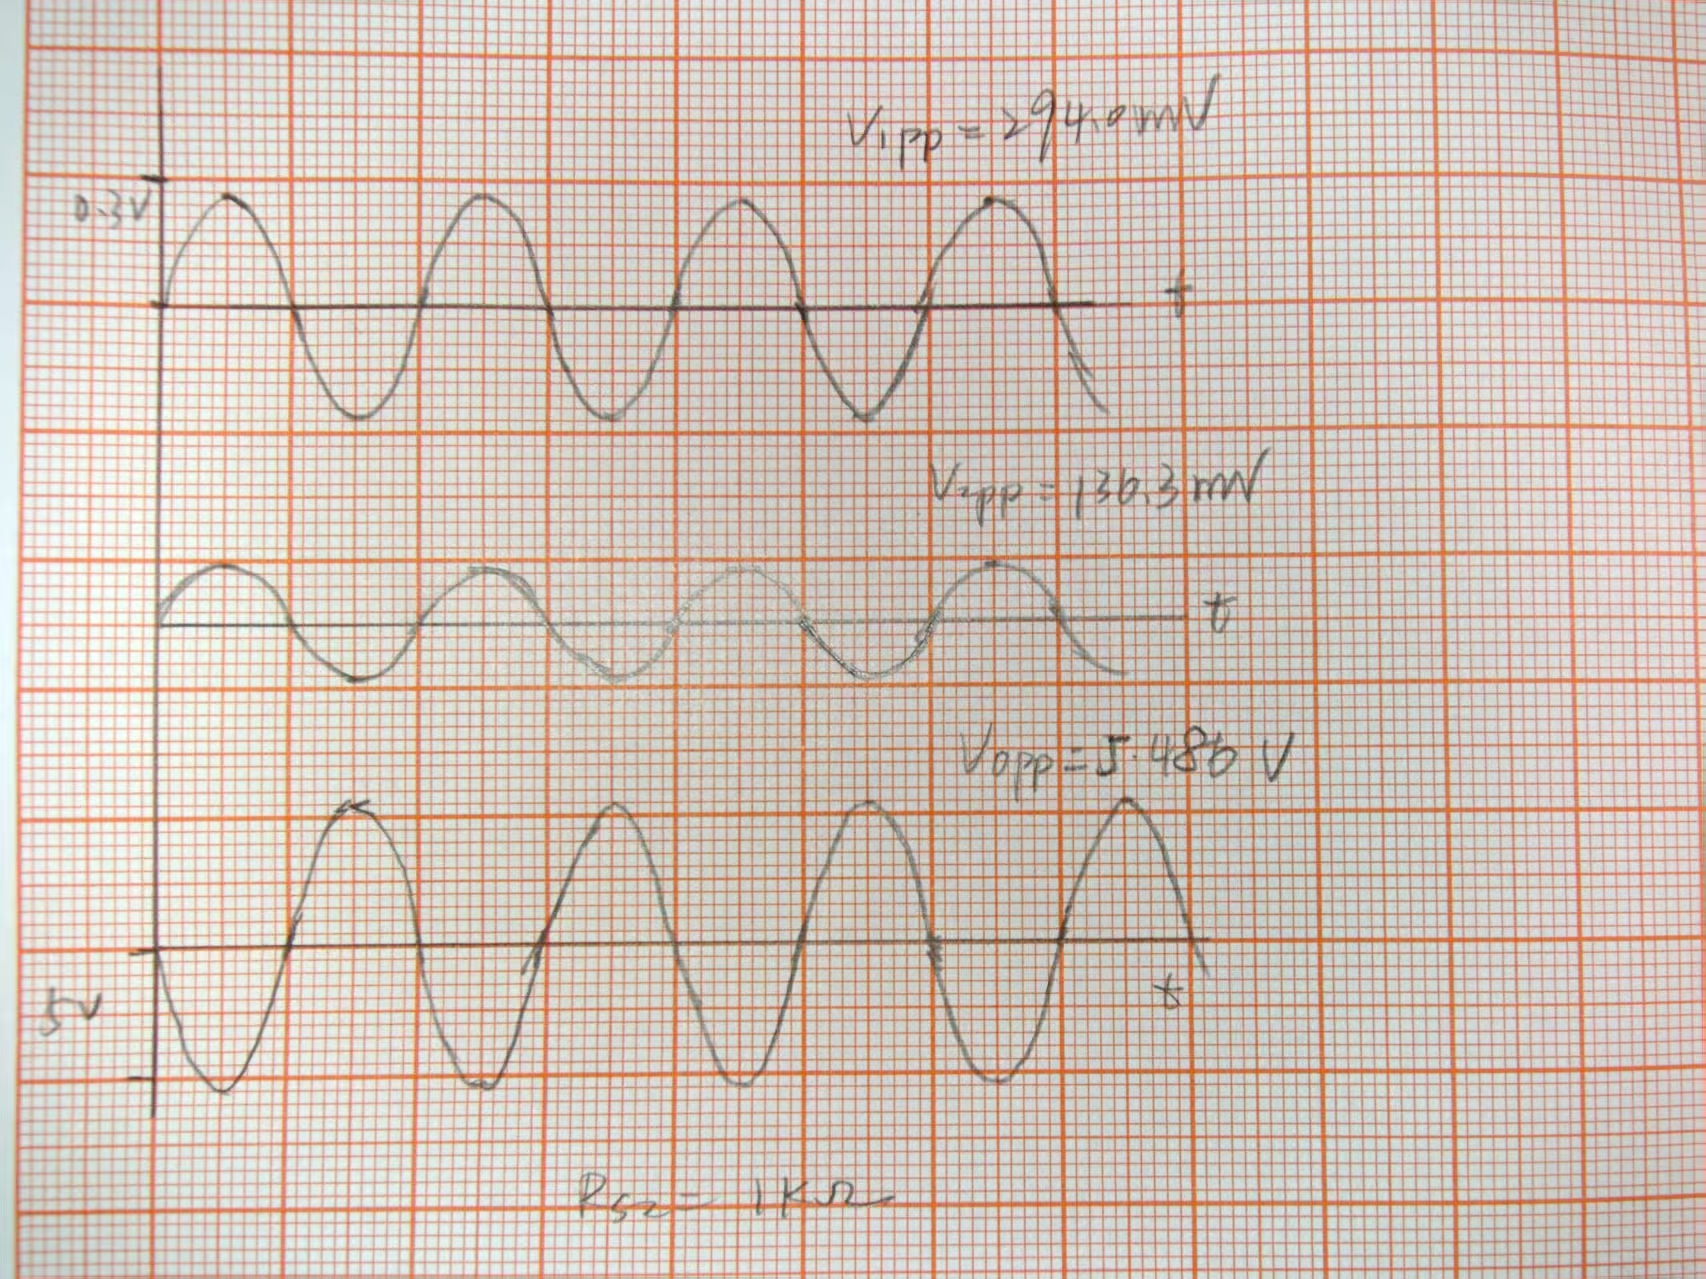
\includegraphics[width=0.45\textwidth]{1.8.jpg}
	}
	\subfigure[$v_{1pp}$,$v_{2pp}$ 和 $v_{opp}$ ($R_{s2}= 500\Omega$)]{
		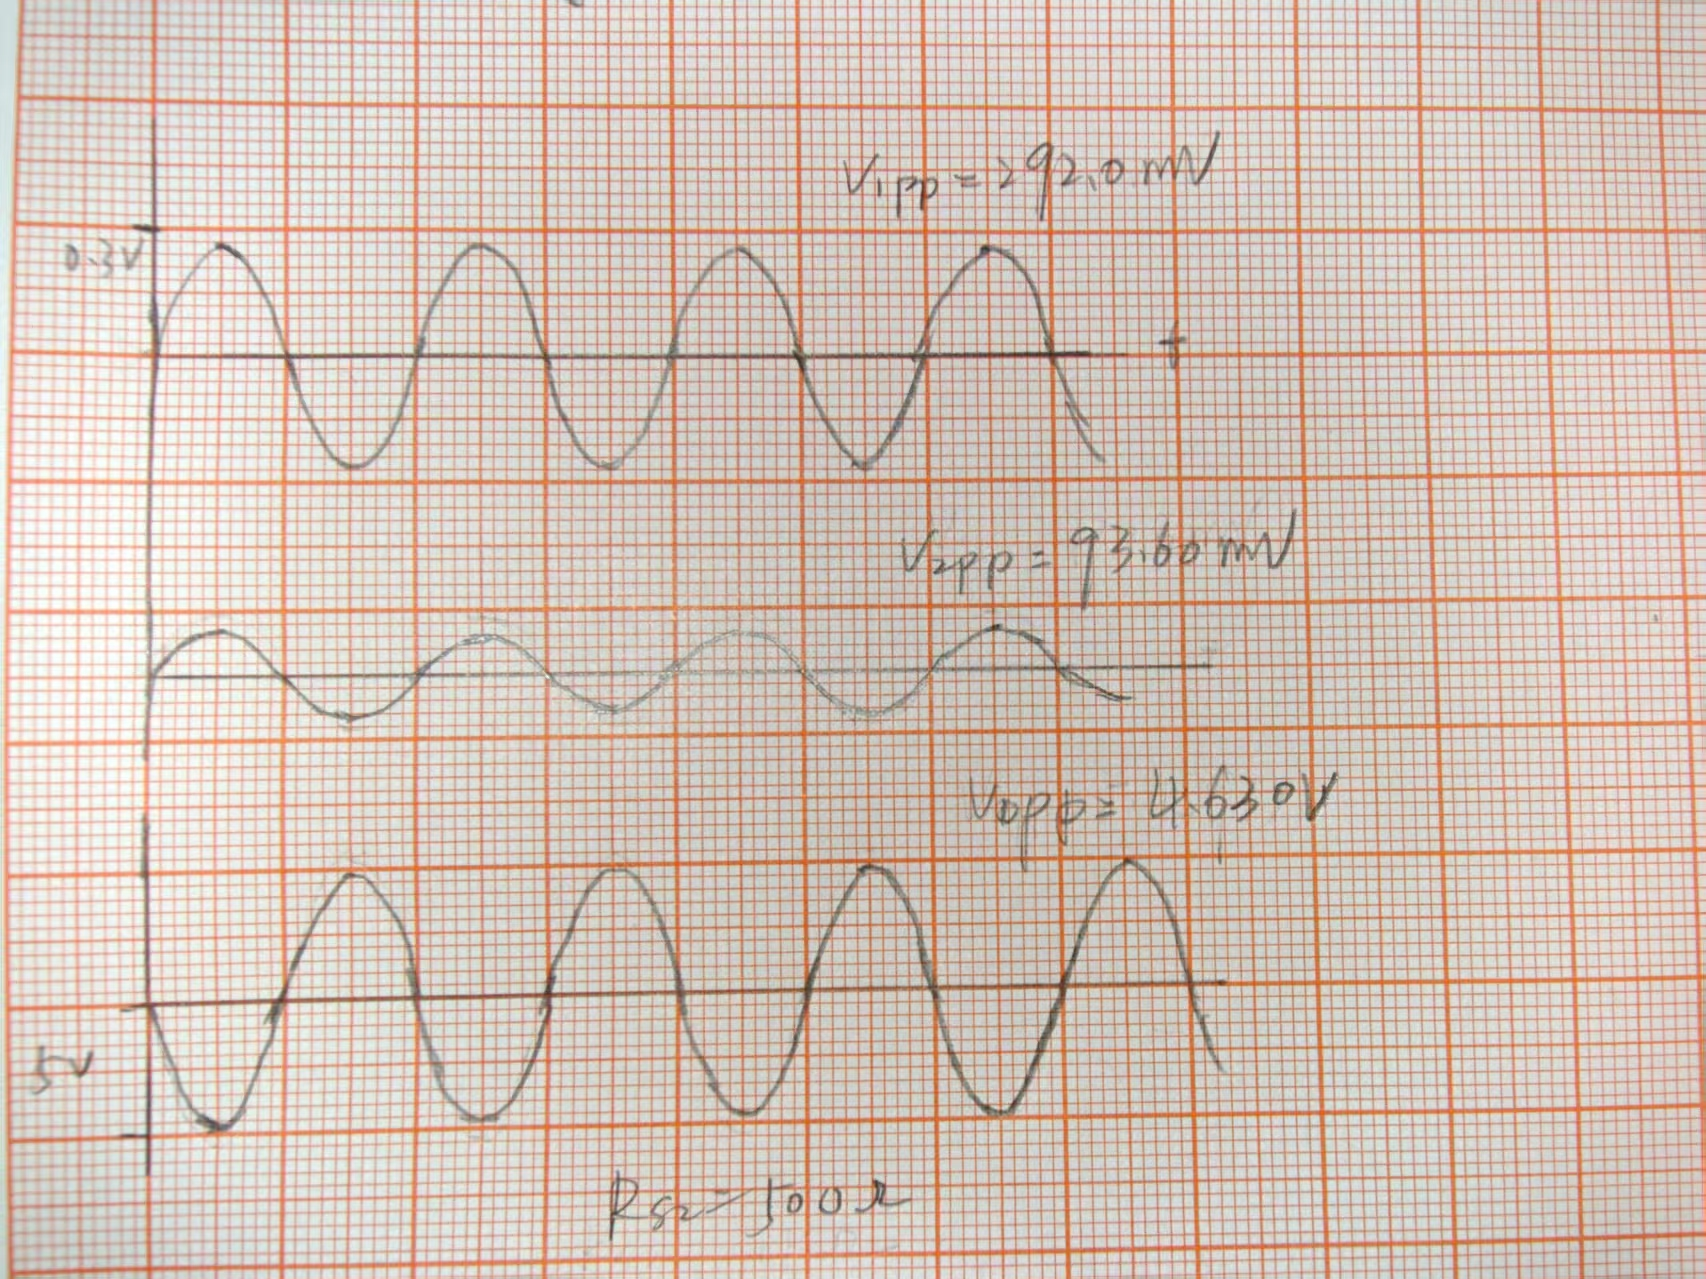
\includegraphics[width=0.45\textwidth]{1.9.jpg}
	}
	\caption{加法器波形图}
\end{figure}

\subsection{任务3: 比例积分电路测试}
观察到的波形如下,基本符合要求:

\begin{figure}[H]
	\centering
	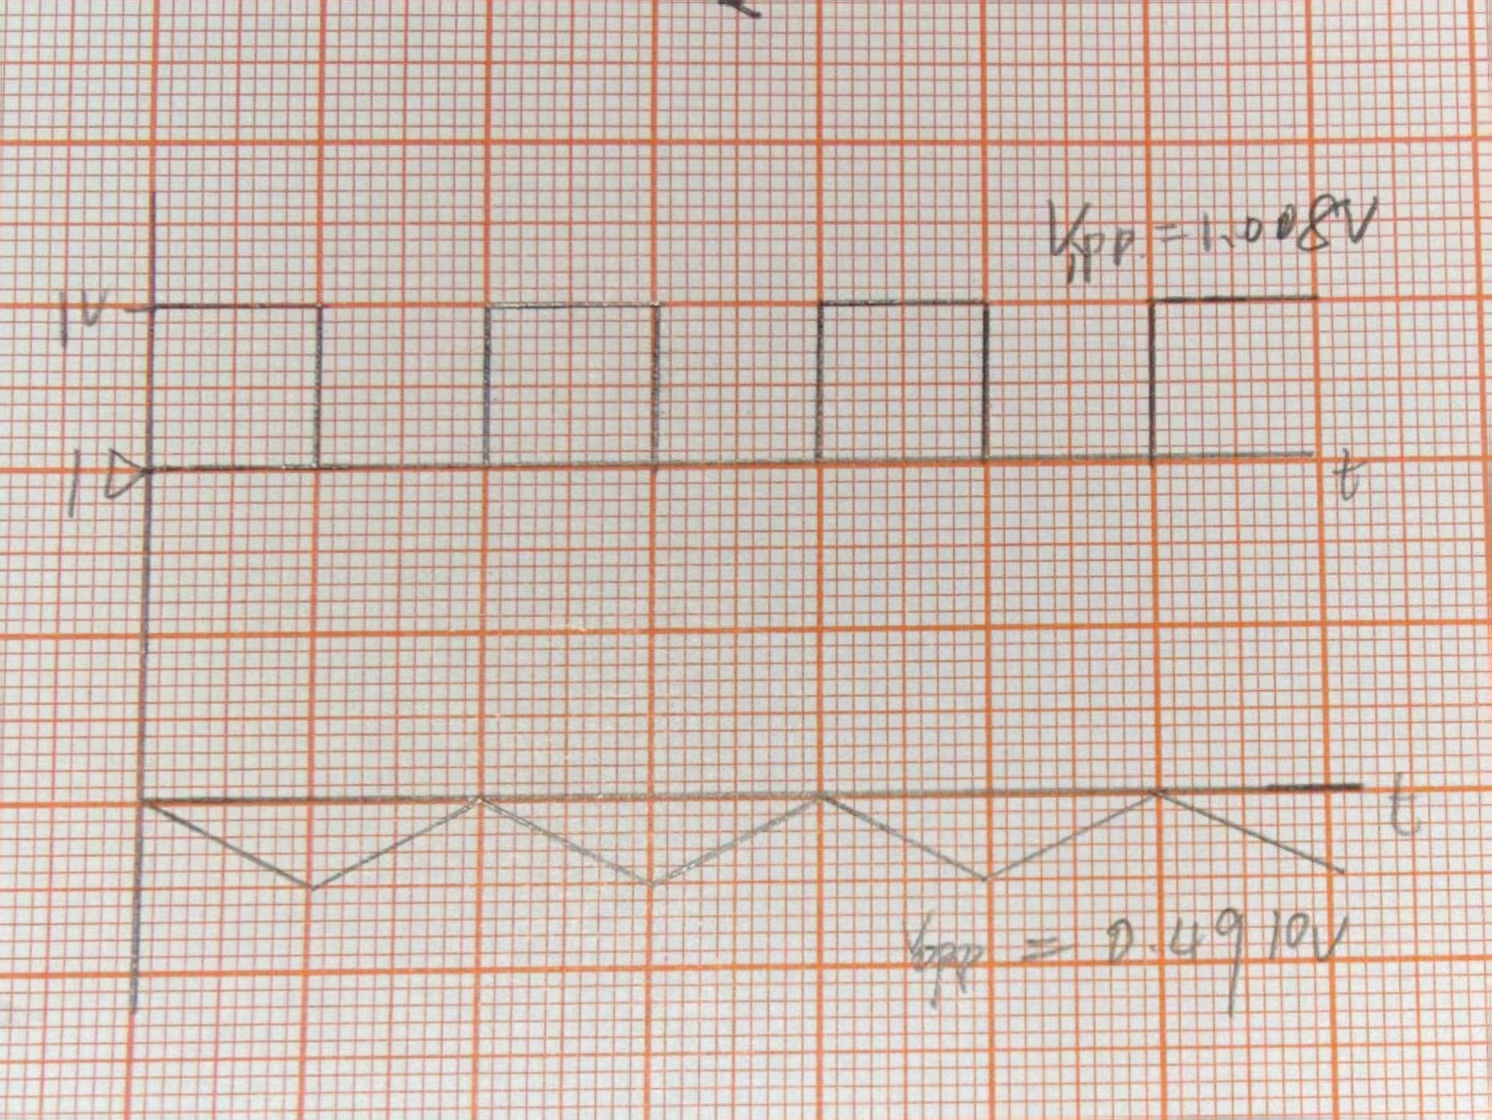
\includegraphics[width=0.8\textwidth]{1.10.jpg}
	\caption{比例积分电路}
\end{figure}

\subsection{任务4: 研究交流仪表放大器的性能}
共模电压增益测量数据如下:

\begin{table}[htbp]
    \centering
    \caption{共模电压增益}
    \label{lable5}
    \begin{tabular}{|c|c|c|}
        \hline
        \multicolumn{2}{|c|}{实测} & 计算(包含相位关系) \\
        \hline
        $v_{icpp}$/V & $v_{ocpp}$/V & $A_{VC}$ \\
        \hline
        9.8 & 0.14 & 0.014\\
        \hline
    \end{tabular}
\end{table}

差模电压增益

\section{实验总结}
本次实验是我的第一次模电实验,学会了实验室中信号源、示波器、电源的使用方法,基本掌握了
运算放大器NE5532的使用原理和接线方法,基本完成了实验要求

\end{document}